\chapter{前提知識}
\label{chap:prerequisite}
本章では,まず深層状態空間モデル(Deep State Space Model, 以下DSSM)のベースとなる変分自己符号化器(Variational Auto Encoder, 以下VAE)について説明し,続いてDSSMの説明を行う

\section{変分自己符号化器(VAE)}
\label{section:VAE}

\begin{figure}[tbp]
\begin{center}
  \begin{tikzpicture}[scale=1, transform shape]
    \node[obs] (x1) {$\bm{x}$};
    \node[latent, above=of x1] (z1) {$\bm{z}$};
    \edge {z1} {x1};
    \end{tikzpicture}
\caption{VAEのグラフィカルモデル}
\label{fig:gm_vae}
\end{center}
\end{figure}

{\bf 変分自己符号化器}({\bf Variational Auto-encoder}, 以下{\bf VAE})\cite{vae}は,深層生成モデルの一種である.
VAEでは,データ$\bm{x} \in \mathbb{R}^n$はある潜在変数$\bm{z} \in \mathbb{R}^m$から生成されると考え,その確率的生成過程$p(\bm{x}|\bm{z})$を多層ニューラルネットワークを用いてモデル化する.
つまり,Fig. \ref{fig:gm_vae}のようなグラフィカルモデルで表現される確率モデルを仮定し,そのパラメータ$\theta$をニューラルネットワークのパラメータとして表現する.
データ$\bm{x}$は手書き数字の画像に該当するが,これはそれぞれの要素が1つのピクセルの値に相当する$28\times28=784$次元のベクトルで表された高次元な表現である.
潜在変数$\bm{z}$は,データ$\bm{x}$をより低次元に表現する.
これは,画像のような高次元なデータは画像空間上の非常に限られた領域に局所的に存在しており,それらはより低次元に表現可能であるとする多様体仮説に基づいている.

すると,データの分布$p(\bm{x})$は,$\theta$によってパラメータ化された条件付き分布$p(\bm{x}| \bm{z}; \theta)$を用いて,
\begin{equation}
p(\bm{x}) = \int p(\bm{x}|\bm{z};\theta) p(\bm{z}) d\bm{z} \label{eq:vae}
\end{equation}
と書くことができる.
%ここで,$p(\bm{x}| \bm{z}; \theta)$は潜在変数からデータを生成するため,デコーダと呼ばれる.
VAEでは,潜在変数の分布について,以下の2つの仮定を置く.
\begin{eqnarray}
p(\bm{z}) &=& \mathcal{N}(\bm{z}|0,\bm{I}) \label{eq:z}\\
p(\bm{z}|\bm{x}) &=& \mathcal{N}(\bm{z}|\mu(\bm{x}),\sigma(\bm{x}))	\label{eq:z_cond}
\end{eqnarray}
式(\ref{eq:z})は,潜在空間が標準正規分布に従っているという仮定であり,式(\ref{eq:z_cond})は,$\bm{x}$に条件づけられた潜在変数の分布が正規分布に従うという仮定である.
ベイズ統計では$p(\bm{z})$は事前分布と呼ばれ,データ$\bm{x}$を観測した後の分布$p(\bm{z}|\bm{x})$は事後分布と呼ばれる.
%また,潜在変数を観測データから推定することを,推論(inference)と呼ぶ.
%$p(\bm{z}|\bm{x})$は,データを低次元の潜在空間に埋め込むため,エンコーダと呼ばれる.
$p(\bm{z}|\bm{x})$を解析的に求めることができるケースは非常に限られており,これが解けない場合,近似分布$q(\bm{z}|\bm{x})$を導入して$p(\bm{z}|\bm{x})$を近似することがベイズ統計ではよく行われる.
VAEでも,$p(\bm{z}| \bm{x})$を別のパラメータ$\phi$を用いて$q(\bm{z}|\bm{x};\phi)$によって近似する.
$p(\bm{z}|\bm{x})$はガウス分布を仮定しているため,$q(\bm{z}|\bm{x};\phi)$もガウス分布を仮定する.
VAEでは,この近似分布$q(\bm{z}|\bm{x};\phi)$もニューラルネットワークを用いて表現する.
%VAEはエンコーダとデコーダの両者をニューラルネットワークで定義する.

\begin{figure}[tbp]
  \begin{center}
    \begin{tikzpicture}[scale=1, transform shape]
      \node[obs] (x1) {$\bm{x}$};
      \node[latent, above=of x1] (z1) {$\bm{z}$};
      \draw (x1) edge[out=135,in=225,->,dashed] (z1);
      \edge {z1} {x1};
      \end{tikzpicture}
  \caption{推論分布を導入したVAEのグラフィカルモデル.実線は生成モデル,点線は推論モデルを示す.}
  \label{fig:gm_vae_inference}
  \end{center}
  \end{figure}


VAEの目的はデータの分布$p(\bm{x})$を推定することであるため,目的関数は式(\ref{eq:vae})の尤度を最大化することである.
しかし,式(\ref{eq:vae})は$\bm{z}$の周辺化を含み,これを解析的に求めることは困難であるため,尤度そのものを計算することはできない.
%そこで,$\theta$によってパラメータ化されたデコーダ$p(\bm{x}|\bm{z}; \theta)$と,$\phi$によってパラメータ化されたエンコーダ$q(\bm{z}|\bm{x};\phi)$を用いて,式(\ref{eq:vae})の対数をとって,その変分下限を次のように導出する.
そこで,式(\ref{eq:vae})に先ほど定義した$p(\bm{z}|\bm{x})$の近似分布$q(\bm{z}|\bm{x};\phi)$を導入し,その対数をとることで,以下のような変分下限を導出する.
\begin{eqnarray}
\log p(\bm{x}) &=& \log \int p(\bm{x}|\bm{z}; \theta) p(\bm{z}) d\bm{z} \nonumber \\
&=& \log \int q(\bm{z}|\bm{x}; \phi) \frac{p(\bm{x}|\bm{z}; \theta) p(\bm{z})}{q(\bm{z}|\bm{x}; \phi)} d\bm{z} \nonumber \\
&\geq& \int q(\bm{z}|\bm{x}; \phi) \log \frac{p(\bm{x}|\bm{z}; \theta) p(\bm{z})}{q(\bm{z}|\bm{x}; \phi)} d\bm{z} \label{eq:jensen}\\
&=& \int q(\bm{z}|\bm{x}; \phi) \log p(\bm{x}|\bm{z}; \theta) d\bm{z} - \int q(\bm{z}|\bm{x}; \phi) \log \frac{q(\bm{z}|\bm{x}; \phi)}{p(\bm{z})} d\bm{z} \nonumber \\
&=& \mathbb{E}_{\bm{z} \sim q(\bm{z}|\bm{x}; \phi)} [\log p(\bm{x}|\bm{z}; \theta)] - \mathrm{D_{KL}}(q(\bm{z}|\bm{x}; \phi) \| p(\bm{z})) \label{eq:elbo}
\end{eqnarray}
ここで,式(\ref{eq:jensen})でイェンセンの不等式(Jensen's inequality)を用いている.
式(\ref{eq:elbo})の第2項の$\mathrm{D_{KL}}$(カルバックライブラー距離)は,いま$p(\bm{z})$,$q(\bm{z}|\bm{x}; \phi)$共にガウス分布を仮定しているため,解析的に計算することができる.
一方,式(\ref{eq:elbo})の第1項は,解析的には計算できないため,$q(z|x; \phi)$からサンプリングされる$L$個の$\bm{z}$を用いて$\frac{1}{L} \sum_{l} \log p(\bm{x}|\bm{z})$でモンテカルロ近似する.通常,$p(\bm{x}|\bm{z})$はベルヌーイ分布や正規分布とし,その尤度を計算する.
VAEではこの変分下限を目的関数として最大化するように,誤差逆伝播法でニューラルネットワークのパラメータ$\theta$と$\phi$の最適化を行う.
しかし,ここで$q(\bm{z}|\bm{x}; \phi)$からサンプリングを行う部分で勾配の計算ができず,計算グラフが途切れてしまって,誤差逆伝搬法を用いた最適化ができなくなってしまうという問題が生じる.
これを解決するために,VAEでは{\bf 再パラメータ化トリック}({\bf reparameterization trick})を使用する.
%Fig. \ref{fig:reparam}に,再パラメータ化トリックの概略を示す.
通常のサンプリングを行う場合,正規分布$q(\bm{z}|\bm{x}; \phi)$の母数である平均$\mu (\bm{x})$と標準偏差$\sigma (\bm{x})$がニューラルネットワークによって出力された後,$N(\mu (\bm{x}), \sigma (\bm{x}))$から$\bm{z}$をサンプリングするが,これでは計算グラフが途切れてしまう.
そこで,再パラメータ化トリックでは,$\mathcal{N}(\mu (\bm{x}), \sigma (\bm{x}))$から直接サンプリングを行う代わりに,標準正規分布$\mathcal{N}(\bm{0},\bm{I})$からサンプルされる変数$\epsilon$を用いて,$\bm{z}=\mu (\bm{x})+ \epsilon \cdot \sigma (\bm{x})$と計算することによって,計算グラフを途切らせることなく,確率的なサンプリングを可能にする.

\begin{figure}[tbp]
  \begin{center}
    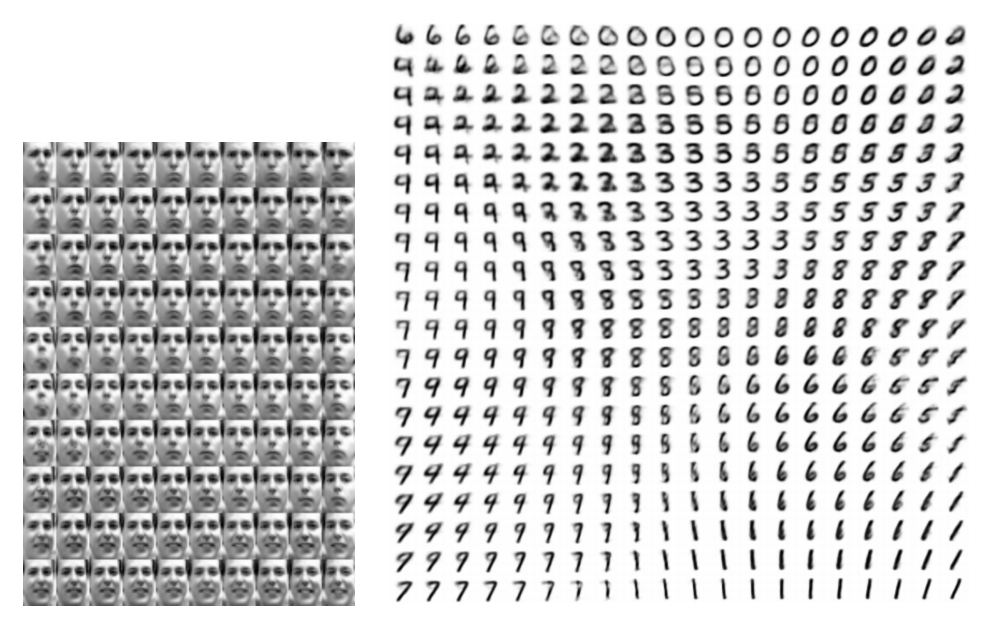
\includegraphics[width=\linewidth]{./figures/vae.png}
    \caption{VAEを用いて生成された画像の例(\cite{vae}より引用)}
    \label{fig:vae}
  \end{center}
\end{figure}

\section{深層状態空間モデル(DSSM)}
\label{section:DSSM}

Non-linear State Space Model, Deep Karman Filters, Deep Markov Model